\chapter{Data Collection}
\label{cha:data_collection}

In this chapter, we provide a comprehensive account of the data collection process
that underpins our experiments. We detail the key steps involved in designing, implementing,
and refining our methodology, with a particular focus on the construction and optimization
of the prompts used to interact with the Large Language Model (LLM).

We begin by presenting the core prompts utilized in our study, describing their
specific applications within each experimental setup. Following this, we outline
the rationale behind our prompt design decisions, grounding our choices in relevant
literature and highlighting key findings from previous research that informed our
approach.

Finally, we introduce the structure of our experimental evaluations, including the
generation of specialized heatmaps designed to illustrate the agent's uncertainty
in action selection. These visualizations provide valuable insights into the
model's decision-making process, highlighting both its generative strengths and areas
for further refinement.

\section{Prompts}
\label{sec:prompts}

This section provides a general overview of the prompts used in our experiments,
while the following one (Section \ref{sec:prompt_creation_choices}) will detail the
specific choices behind each specific part of them. The prompts were designed to
be concise yet comprehensive, ensuring that they effectively elicited the desired
responses from the model.

In the next subsections, we will present two core prompts that formed the
foundation of our experiments. These prompts were specifically designed to assess
the model's ability to generate optimal actions (one at the time) in our two main
tasks: picking up and delivering a parcel.

This section provides a general overview of the prompts used in our experiments.
While the subsequent section (Section \ref{sec:prompt_creation_choices}) delves into
the specific design choices behind each component, here we present the
fundamental structure and intent of the core prompts.

Our prompts were designed to be both concise and comprehensive, ensuring they effectively
guided the model in generating appropriate next-step actions. The core idea was
to elicit responses that incrementally moved the agent toward its objective, either
picking up or delivering a parcel, while minimizing ambiguity in the
instructions.

The two primary prompts used in our study are:
\begin{itemize}
  \item Pickup prompt: guiding the agent to retrieve a parcel from a specified
    location;

  \item Delivery prompt: prompting the agent to transport the parcel to its
    designated drop-off point.
\end{itemize}

Each prompt was carefully structured to provide relevant contextual information
while avoiding unnecessary complexity that could dilute the model's focus.

\subsection{Pickup prompt}

The Pickup prompt (Listing \ref{lst:pickup_prompt}) was used to evaluate the model's
ability to generate actions in the \emph{pickup} scenario. In this setup, the
agent was tasked with picking up a parcel from a specific location on the map. The
prompt provided the agent with the raw map information, including the map
dimensions, the location of the parcel, and the agent's current position.

The model was then asked to determine the optimal next action that would bring
the agent one step closer to the parcel.

\begin{codewindow}
  [Text] \lstset{style=promptstyle, language=prompt, caption={Pickup prompt used in the experiments},
  label={lst:pickup_prompt}} \begin{lstlisting}
You are a delivery agent in a web-based delivery game where the map is a matrix
I am going to give you the raw information I receive from the server and the possible actions.
Map width: {width}
Map height: {height}
Tiles are arranged as {height} rows in {width} columns:
{tiles}
The parcel you need to take is in the spot ({parcelX}, {parcelY}).
You are on the spot ({agentX}, {agentY}).
The actions you can do ONLY if the next tile is available are:
U) move up
D) move down
L) move left
R) move right
T) take the parcel that is in your tile
S) ship a parcel (you must be in a delivery tile)

Your final goal is to go to a tile with the parcel and (T)ake it, I need the best action that will get you there.
Don't explain the reasoning and don't add any comment, just provide the action's letter.
What is your next action?
\end{lstlisting}
\end{codewindow}

\subsection{Deliver prompt}
The Delivery Prompt (Listing \ref{lst:deliver_prompt}) was structured to evaluate
the model's ability to navigate toward a designated drop-off location. Unlike
the Pickup Prompt, where the parcel's position was explicitly provided, the
delivery prompt required the LLM to infer the delivery destination from the map
description. The model was then asked to determine the best next action to move toward
the inferred delivery location.

\begin{codewindow}
  [Text] \lstset{style=promptstyle, language=prompt, caption={Deliver prompt used in the experiments},
  label={lst:deliver_prompt}} \begin{lstlisting}
You are a delivery agent in a web-based delivery game where the map is a matrix
I am going to give you the raw information I receive from the server and the possible actions.
Map width: {width}
Map height: {height}
Tiles are arranged as {height} rows in {width} columns:
{tiles}
You are on the spot ({agentX}, {agentY}).
The actions you can do are:
U) move up
D) move down
L) move left
R) move right
T) take the parcel that is in your tile
S) ship a parcel (you must be in a delivery tile)

You have a parcel to ship, your final goal is to go to the delivery zone (delivery = true) and (S)hip the parcel, I need the best action that will get you there.
Don't explain the reasoning and don't add any comment, just provide the action's letter.
What is your next action?
\end{lstlisting}
\end{codewindow}

\section{Prompt Creation Choices}
\label{sec:prompt_creation_choices}

This section outlines the key considerations that guided the construction of our
prompts (commonly referred to as Prompt Engineering). We describe the reasoning
behind specific design choices, following the sequence in which they appear in the
prompt. For clarity, we use the Pickup Prompt (Listing \ref{lst:pickup_prompt}) as
a reference.

\subsection{Role Prompting}
Assigning specific roles or personas to Large Language Models (LLMs) within prompts,
known as ``role prompting," has been shown to enhance their performance on
various tasks. This technique involves instructing the model to assume a particular
identity, such as a ``math professor" or ``geographer," to guide its responses more
effectively. The concept of role prompting has been explored in several studies.

For instance, the paper `Better Zero-Shot Reasoning with Role-Play Prompting' by
Kong et al. \cite{kong2024betterzeroshotreasoningroleplay} demonstrated that
strategically designed role-play prompts can significantly improve LLMs' reasoning
abilities across diverse benchmarks.

Similarly, `Role-Play Zero-Shot Prompting with Large Language Models for Open-Domain
Human-Machine Conversation' by Njifenjou et al. \cite{njifenjou2024roleplayzeroshotpromptinglarge}
investigated the use of role-play prompts to enhance conversational agents'
performance without additional fine-tuning.

In our experiments, we employed role prompting to encourage the model to adopt the
persona of a \emph{delivery agent}, thereby focusing its attention on the task at
hand. By framing the prompts in this manner, we aimed to guide the model's responses
towards generating coherent and contextually relevant actions.

\subsection{Map Encoding to Reduce Attention Sparsity}

One of our primary concerns was that the map included in the prompt might take
up too much space, which could lead to an excessively sparse distribution of attention.
This could result in the model not properly focusing on crucial aspects of the
input. At the same time, we wanted to maintain a minimal and flexible approach
to map handling. Our goal was to ensure that the system would continue functioning
even if the format of the map-providing function were to change unexpectedly. As
discussed in Section \ref{sub:our_task}, this design decision was made to simulate
an unpredictable and rapidly changing environment.

To address this concern, we first aimed to understand how the model processed
map-related information. Ideally, we would have examined the model’s attention
scores directly, but unfortunately, OpenAI’s API does not provide access to
these scores. As a result, we had to rely on a qualitative analysis instead. To achieve
this, we leveraged BERT, another Transformer-based architecture, to visualize
attention patterns in our original prompt. The results revealed that a significant
portion of the model’s attention was focused on tokens related to JSON syntax rather
than the meaningful content of the prompt itself. This suggested that structural
elements, rather than semantic information, were drawing a disproportionate
amount of attention.

Based on this observation, we attempted to reduce the presence of JSON syntax within
the prompt while preserving the essential information. We then repeated the same
attention analysis using this modified version. The results showed a notable shift
in the distribution of attention. Specifically, when we examined the tokens receiving
the highest attention—excluding punctuation, as well as the special starting and
ending tokens—we found that in the original prompt, only 23 out of the top 50 tokens
were meaningful words. In contrast, in the revised prompt, this number increased
to 31 out of 50, indicating a more focused attention on relevant content.

For this test, we used an older version of the "Pickup prompt," which is explained
in detail in Section \ref{sec:second_approach}. As demonstrated in Table
\ref{tab:prompt_comparison}, the revised version of the prompt not only contained
more words but also explicitly included the term pickup, which is the key focus
of our task. Notably, this term was entirely absent from the top attention-receiving
tokens in the initial prompt.

\begin{table}[h]
  \centering
  \begin{tabular}{|c|c|}
    \hline
    \textbf{Old Prompt} & \textbf{New Prompt} \\
    \hline
    game                & game                \\
    reasoning           & parcel              \\
    parcel              & reasoning           \\
    parcel              & i                   \\
    score               & actions             \\
    response            & you                 \\
    parcel              & if                  \\
    tile                & parcel              \\
    i                   & moves               \\
    if                  & height              \\
    you                 & width               \\
    response            & score               \\
    loop                & ship                \\
    comment             & tile                \\
    information         & loop                \\
    actions             & information         \\
    and                 & choosing            \\
    ship                & you                 \\
    and                 & \textbf{pickup}     \\
    server              & and                 \\
    you                 & you                 \\
    choosing            & parcel              \\
    using               & and                 \\
                        & server              \\
                        & information         \\
                        & and                 \\
                        & ship                \\
                        & explain             \\
                        & using               \\
                        & reward              \\
                        & name                \\
    \hline
  \end{tabular}
  \caption{Comparison of Old and New Prompts}
  \label{tab:prompt_comparison}
\end{table}

To further analyze the impact of this change, we collected attention scores from
both the old and new prompt versions. We then removed the tokens corresponding to
the map representation and plotted the difference between the two distributions.
The resulting visualization is presented in Figure \ref{fig:difference}. Interpreting
this figure is not entirely straightforward, and we acknowledge that it is
unclear to what extent this analysis can serve as a direct proxy for a GPT-based
model. However, one noticeable trend is that the diagonal elements exhibit a
lower overall attention intensity (indicated by the presence of purple and dark blue
regions). Meanwhile, most of the remaining areas show a delta close to zero (represented
in aqua blue), suggesting that the changes we introduced led to a redistribution
of attention without introducing excessive noise or unintended biases.

\begin{figure}[h!]
  \centering
  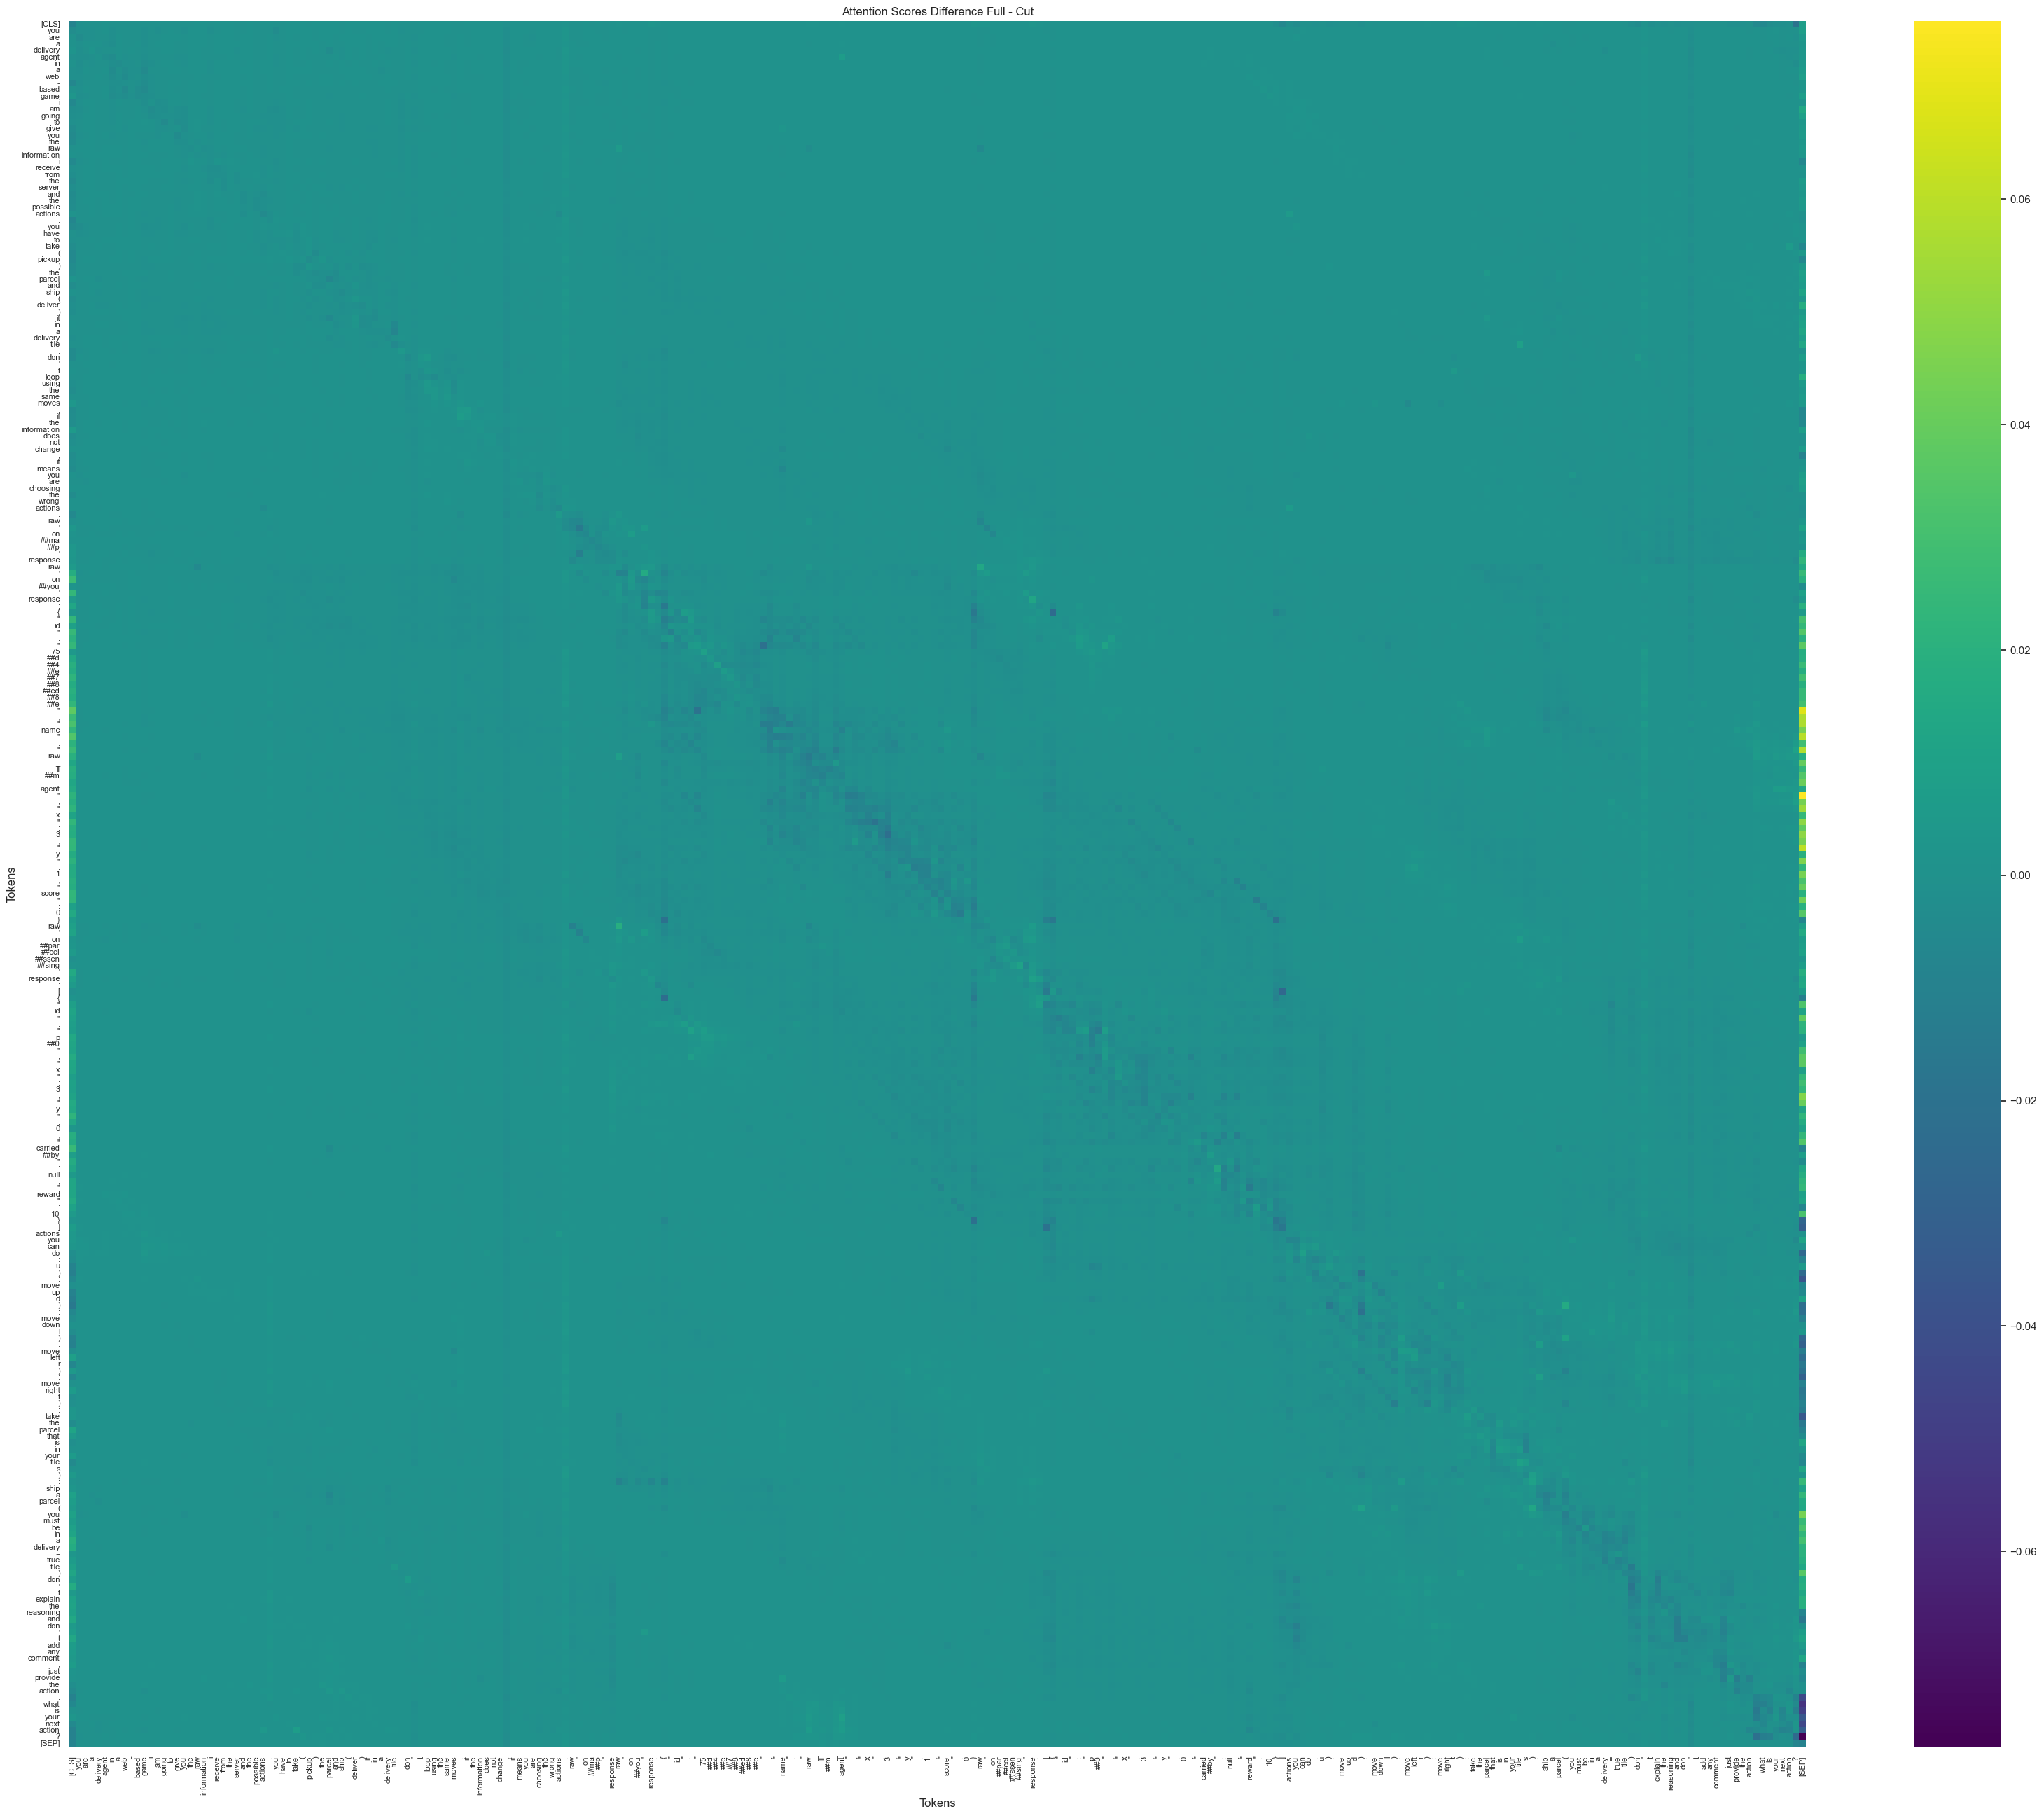
\includegraphics[width=0.8\textwidth]{images/difference.png}
  \caption{Caption}
  \label{fig:difference}
\end{figure}

\subsubsection{Emerging behavior: encoded question decoded answer}

Another strategy we explored to reduce the space occupied by the map in the prompt
was to encode it. Our goal was to compress the map representation while ensuring
that the model could still understand the relevant information.

A relevant study on this topic is presented in the paper `LLMs Can Understand Encrypted
Prompt: Towards Privacy-Computing Friendly Transformers" \cite{liu2023llmsunderstandencryptedprompt}.
The authors of this paper aimed to preserve user privacy by encrypting prompts
before sending them to a language model. Their findings demonstrated that the model
was able to comprehend and respond appropriately to encrypted prompts. This
suggested that LLMs possess an inherent ability to process encoded text
meaningfully.

Inspired by these results, we conducted an experiment to determine whether a similar
encoding approach could be used to reduce the space occupied by the map while preserving
its usability within the prompt. Specifically, we investigated whether the model
could still interpret a compressed version of the map if it were encoded.

To validate this, we first examined the model's ability to process encoded
prompts by testing a simple case. As shown in Figure \ref{fig:b64gpt}, the model
successfully understood the meaning of the question "Can you tell me how many apples
remain and their color if I have two red apples and two green apples and I eat one
of both?" even when the entire prompt was encoded in BASE64 (see Figure
\ref{fig:texttob64}). Notably, the model did not generate a decoding function before
answering. Instead, it directly processed the encoded prompt and returned a response
in plain English, demonstrating its ability to work with BASE64-encoded text.

Encouraged by these results, we attempted to apply a similar encoding strategy to
the map representation while also aiming to reduce the number of characters in the
prompt. Our hypothesis was that reducing the character count would also reduce
the number of tokens, thereby improving attention efficiency.

To test this, we implemented a two-step encoding process in Python, as outlined in
Listing \ref{lst:double_enc}:
\begin{enumerate}
  \item First, we compressed the map using the \texttt{zlib} library and its Deflate
    algorithm \footnote{\url{https://en.wikipedia.org/wiki/Deflate}} to minimize
    its size;

  \item Next, we encoded the compressed output in BASE64 \footnote{\url{https://en.wikipedia.org/wiki/Base64}}
    using the \texttt{base64} library;

  \item Finally, we inserted this doubly encoded map into the prompt.
\end{enumerate}

\vspace{10mm}
\begin{codewindow}
  [Python Code] \lstset{style=pythonstyle, language=Python, caption={Example of double encoding algorithm},
  label={lst:double_enc}} \begin{lstlisting}
[...]

input_string = MAP
compressed_data = zlib.compress(input_string.encode('utf-8'))
compressed_base64 = base64.b64encode(compressed_data).decode('utf-8')

[...]
\end{lstlisting}
\end{codewindow}
\vspace{10mm}

While this method did succeed in reducing the number of characters by X\%, the
results were not as expected in terms of model comprehension. Unlike the case of
simple BASE64 encoding, the LLM was no longer able to interpret the prompt
correctly. Instead, its responses typically fell into one of two categories:
\begin{itemize}
  \item The model would explicitly state that it recognized the input as an encrypted
    message and ask: ``I see you sent me an encrypted message. Do you want me to
    decrypt it?";

  \item Alternatively, the model would generate a Python function to decode the
    input before attempting to process it. This behavior likely stemmed from the
    fact that our encoding method—using zlib compression followed by BASE64 encoding—is
    a well-known and widely used technique on the internet. As a result, the model
    had encountered similar patterns in its training data and inferred that the input
    should first be decoded before use.
\end{itemize}

Furthermore, although our approach successfully reduced the total number of characters
in the prompt, it did not achieve our ultimate objective. Counterintuitively,
the number of tokens actually increased rather than decreased. This is because tokenization
in LLMs is based on common character sequences rather than individual characters.
Encoding the map disrupted these common patterns, leading to a tokenization process
that resulted in a higher overall token count. Consequently, the intended effect
of reducing attention sparsity was not achieved, as illustrated in Figure
\ref{fig:lesscharmoretokens}.

In summary, while encoding techniques like BASE64 alone might be useful for preserving
meaning in certain contexts, our specific approach of compressing and encoding
the map did not lead to the desired efficiency gains. Instead, it introduced
additional computational overhead and interpretation challenges for the model, ultimately
making this approach ineffective for our purposes.

\begin{figure}[h!]
  \centering
  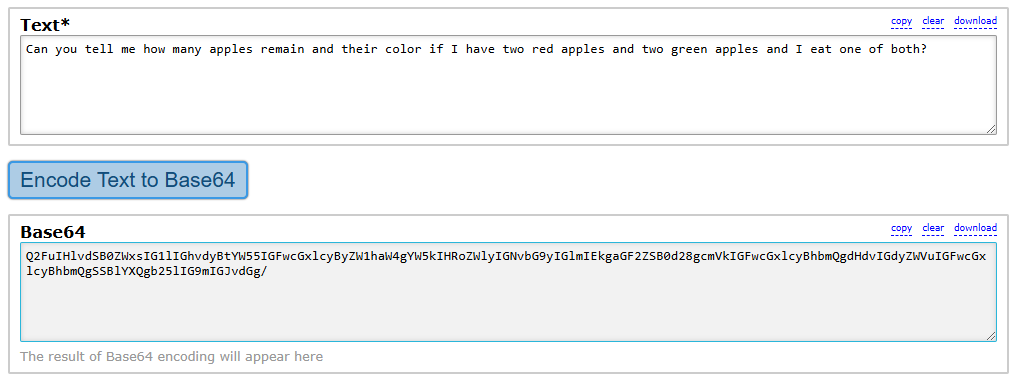
\includegraphics[width=0.8\textwidth]{images/texttob64.png}
  \caption{Caption}
  {Source: https://base64.guru/converter/encode/text} \label{fig:texttob64}
\end{figure}

\begin{figure}[h!]
  \centering
  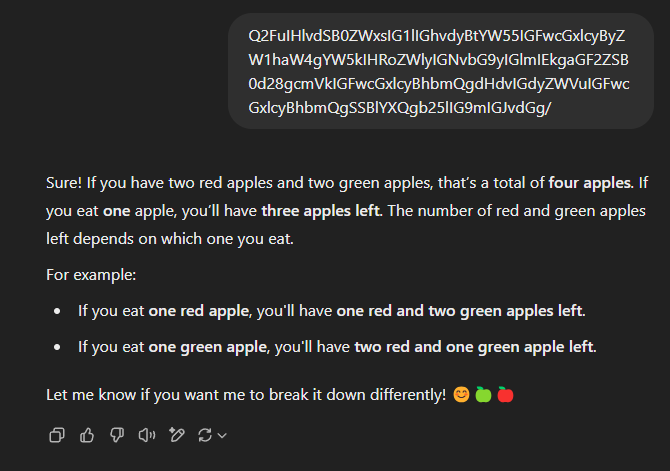
\includegraphics[width=0.8\textwidth]{images/b64gpt.png}
  \caption{Caption}
  {Source: GPT-4o via OpenAI website} \label{fig:b64gpt}
\end{figure}

\subsection{Emerging behavior: math capabilities}

We also investigated the impact of including action-related information, such as
explicitly stating ``Going up increases your X position by 1" for every movement
action. It initially seemed like a promising way to guide the model's reasoning.
However, this conflicted with our overarching goal of keeping the system adaptable
rather than grounding it in a fixed environmental structure. Despite this, we proceeded
with the experiment to assess its impact.

Interestingly, we observed that the model's performance in navigation tasks was
unexpectedly strong, even to the point of raising concerns about potential shortcuts.
To further investigate, we conducted a follow-up test in which we entirely removed
the map from the prompt. As result, the model still produced correct answers by seemingly
ignoring any extraneous details and reducing the problem to simple arithmetic.
It recognized that if the starting position was \texttt{(4,3)} and the goal was at
\texttt{(0,0)}, the necessary movement was simply decreasing \texttt{X} by 4 and
\texttt{Y} by 3. This behavior demonstrated that the model could abstract away the
spatial representation and ``cheating'' by operating purely on mathematical reasoning.

This finding aligns with existing research on the emergent mathematical reasoning
capabilities of large language models. For example, Wei et al. highlight how
LLMs exhibit "emergent abilities", capabilities that do not appear in smaller models
but spontaneously manifest as model scale increases \cite{wei2022emergentabilitieslargelanguage}.
Among these abilities, arithmetic and mathematical reasoning are particularly notable,
suggesting that LLMs can generalize numerical patterns without explicit training
for such tasks. Our experiment provides anecdotal evidence supporting this:
rather than relying on the environmental constraints provided in the prompt, the
model instinctively leveraged its inherent mathematical capabilities to deduce the
necessary movements.

Ultimately, given this behavior, we abandoned the idea of including the results of
the actions in the prompt.

\subsection{Question structure}

In know no, they say ENV + LIST OF ACTIONS +``Which option is correct? Answer with
a single letter.''

This approach is also used by some benchmarks to evaluate the performance of language
models on specific tasks \footnote{https://en.wikipedia.org/wiki/MMLU}.

\subsection{Goal positioning}

The goal was at the end due to [golden needle], that says that LLMs tend to focus
on the last part of the prompt.

\section{Leveraging Prompt Caching}
As can be seen in Listing \ref{lst:deliver_prompt} and Listing \ref{lst:pickup_prompt},
the ``changing part" of the prompt, such as the position of the agent, was placed
at the end, while the main static components, including the role and map, were
positioned at the top. This structure was intentionally designed to take advantage
of OpenAI's prompt caching API\footnote{\url{https://platform.openai.com/docs/guides/prompt-caching}}.

According to OpenAI's documentation, for any prompt exceeding 1000 tokens, only
the modified portion is recomputed, while the cached static portion remains unchanged.
This significantly improves efficiency by reducing computational overhead, resulting
in faster response times and lower operational costs. The benefits of this
approach are especially pronounced in the stateful version of the agent, where the
LLM receives the entire conversation history with each request. In this case, caching
allows the model to handle long, continuous interactions without constantly
reprocessing the entire history from scratch, making the system much more scalable
and responsive.

By structuring prompts in this manner, we ensure that also queries for the
stateful agent benefit from caching, leading to optimized performance in our scenario
that required frequent API calls.

\section{Heatmap Generation}
\label{sec:heatmap_generation}

What are, how they are generated, how to read them, why they are useful. How
they are organized in the repo.

Last, we considered the orientation of the map included in the prompts. While
the specific details of this analysis will be discussed in the Results and
Discussion chapter, it is worth noting that the way the map is presented to the model
shows a bias towards a specific orientation (a programming matrix and not a
cartesian plane).